\setAuthor{Päivo Simson}
\setRound{piirkonnavoor}
\setYear{2023}
\setNumber{G 7}
\setDifficulty{7}
\setTopic{TODO}

\prob{Voltmeeter}
\begin{wrapfigure}{r}{0.35\textwidth}
  \begin{center}
    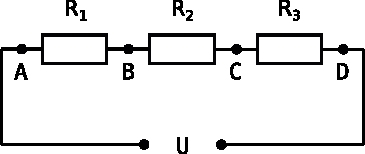
\includegraphics[width=1\linewidth]{2023-v2g-07-yl.pdf}
  \end{center}
  \vspace{-2em}
\end{wrapfigure}

Kolm tundmatut takistit on ühendatud jadamisi ja neile on rakendatud pinge $U=\SI{126}{\volt}$. Tundmatu sisetakistusega voltmeetriga mõõdetakse pingeid joonisel näidatud punktide vahel. Tulemuseks on näidud $V_{AB}=V_{CD}=\SI{28}{\volt}$ ja $V_{AC}=\SI{84}{\volt}$. Millist pinget näitab voltmeeter, kui selle klemmid ühendada punktidega B ja C?




\hint

\solu
Olgu voltmeetri sisetakistus $R_v$. Skeemi sümmeetriast ja võrdusest $V_{AB}=V_{CD}$ järeldub, et takistused $R_1$ ja $R_3$ peavad olema võrdsed, st $R_3=R_1$. \p{1}

\begin{wrapfigure}{r}{0.35\textwidth}
\vspace{-1em}
  \begin{center}
    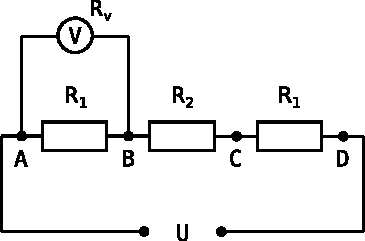
\includegraphics[width=1\linewidth]{2023-v2g-07-sol1.pdf}
  \end{center}
\end{wrapfigure}

1) Koostame kõigepealt skeemi, mis kujutab pinge mõõtmist punktide A ja B vahel. $R_v$ ja $R_1$ on ühendatud rööbiti ja takistus punktide A ja B vahel on järelikult
\[
R_{AB}=\frac{R_v R_1}{R_v + R_1}. \quad \p{0,5}
\]
Skeemi kogutakistus on
\[
R_{k}=\frac{R_v R_1}{R_v + R_1} + R_1+R_2. \quad \p{0,5}
\]
Pinge kahe punkti vahel jaotub proportsionaalselt nende punktide vahelise takistusega ja järelikult
\begin{multline*}
V_{AB}=U\cdot\frac{R_{AB}}{R_k}=\frac{U\frac{R_v R_1}{R_v + R_1}}{\frac{R_v R_1}{R_v + R_1} + R_1+R_2}=\\
=\frac{UR_vR_1}{R_v(2R_1+R_2)+R_1(R_1+R_2)}. \quad \p{1}
\end{multline*}

\begin{wrapfigure}{r}{0.35\textwidth}
\vspace{-1em}
  \begin{center}
    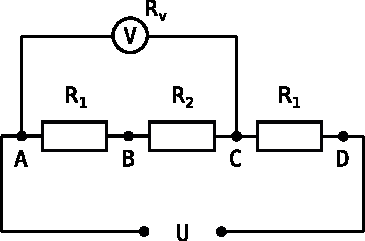
\includegraphics[width=1\linewidth]{2023-v2g-07-sol2.pdf}
  \end{center}
\end{wrapfigure}

2) Koostame skeemi, mis kujutab pinge mõõtmist punktide A ja C vahel. Analoogiliselt eelmise skeemiga saame
\[
R_{AC}=\frac{R_v (R_1+R_2)}{R_v + R_1+R_2}, \quad \p{0,5}
\]
\[
R_{k}=\frac{R_v (R_1+R_2)}{R_v + R_1+R_2}+R_1, \quad \p{0,5}
\]
\begin{multline*}
V_{AC}=U\cdot\frac{R_{AC}}{R_k}=\frac{U\frac{R_v (R_1+R_2)}{R_v + R_1+R_2}}{\frac{R_v (R_1+R_2)}{R_v + R_1+R_2}+R_1}=\\
=\frac{UR_v(R_1+R_2)}{R_v(2R_1+R_2)+R_1(R_1+R_2)}. \quad \p{1}
\end{multline*}

3) Paneme tähele, et $V_{AB}$ ja $V_{AC}$ murdavaldiste nimetajad on samad. Jagame need avaldised omavahel.
\[
\frac{V_{AB}}{V_{AC}}=\frac{R_1}{R_1+R_2}=\frac{28}{84}=\frac{1}{3} \quad\implies\quad R_2=2R_1. \quad \p{2}
\]
Asendades saadud tulemuse $V_{AB}$ avaldisse saame
\[
\frac{126 R_v}{4R_v+3R_1}=28\quad\implies\quad R_v=6R_1. \quad \p{2}
\]

\begin{wrapfigure}{r}{0.35\textwidth}
\vspace{-2em}
  \begin{center}
    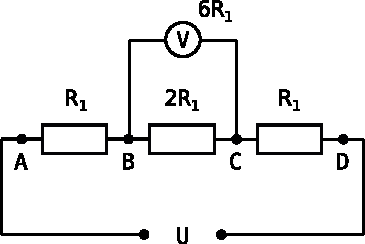
\includegraphics[width=1\linewidth]{2023-v2g-07-sol3.pdf}
  \end{center}
\vspace{-5em}
\end{wrapfigure}

4) Nüüd saame leida voltmeetri näidu $V_{BC}$. Vastavalt skeemile saame
\begin{multline*}
V_{AB}=U\cdot\frac{R_{BC}}{R_k}=\SI{126}{V}\cdot\frac{\frac{2R_1\cdot6R_1}{8R_1}}{\frac{2R_1\cdot6R_1}{8R_1}+2R_1}=\\
=\SI{126}{V}\cdot\frac{12}{12+8\cdot2}=\SI{54}{V}. \quad \p{1}
\end{multline*}
\probend